\documentclass{article}
\usepackage{tikz}
\usetikzlibrary{shapes, arrows}

\begin{document}
\title{Propuesta para historia de datos}
\date{}
\maketitle

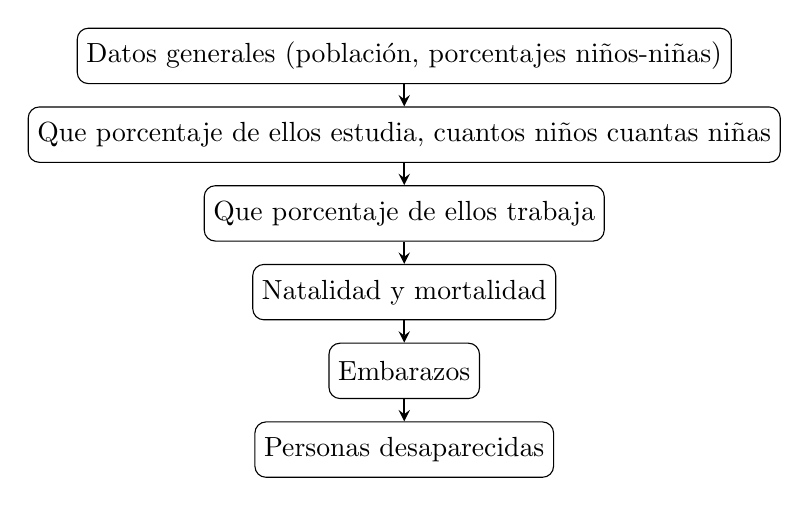
\begin{tikzpicture}

\tikzstyle{terminator} = [rectangle, draw, text centered, rounded corners, minimum height=2em]
\tikzstyle{arrow} = [thick,->,>=stealth]

\node (start) [terminator] {Datos generales (población, porcentajes niños-niñas)};

\node (segundo) [terminator, below of=start] {Que porcentaje de ellos estudia, cuantos niños cuantas niñas};

\node (trabajo) [terminator, below of=segundo] {Que porcentaje de ellos trabaja};

\node (natalidad) [terminator, below of=trabajo] {Natalidad y mortalidad};

\node (fecundidad) [terminator, below of=natalidad] {Embarazos};
\node (personas desaparecidas) [terminator, below of=fecundidad] {Personas desaparecidas};

\draw [arrow] (start) -- (segundo);
\draw [arrow] (segundo) -- (trabajo);
\draw [arrow] (trabajo) -- (natalidad);
\draw [arrow] (natalidad) -- (fecundidad);
\draw [arrow] (fecundidad) -- (personas desaparecidas);

\end{tikzpicture}
\end{document}